\documentclass{article}
\usepackage[utf8]{inputenc}
\usepackage{english}
\usepackage{footnote}
\usepackage{graphicx}
\usepackage{bbding}
\usepackage{pifont}

\setlength{\parskip}{1em}

\title{\textbf{Big Data report} \\ \vspace{2em} team: Magiczny Krzysztof \\ \vspace{2em}}
\author{Spaliński Krzysztof, \\ Kała Jakub, \\ Dyczko Michał, \\ Pawłowski Maciej}
\date{\vfill March 2020}


\begin{document}

\clearpage\maketitle
\thispagestyle{empty}

\newpage

\section{Project description}

% Krótki opis celu projektu z perspektywy odbiorcy rozwiązania,
% czyli wysokopoziomowy opis produktu (produktów) projektu
% Strona do analizy memów w internecie. Dwa oddzielne aspekty:
% 1. Analiza tematów (word2vec + klasteryzacja)
% 2. Analiza formatów memów (klasteryzacja) + linki do strony knowyourmeme.com

% Źródłem danych będą popularne strony z memami takie jak reddit oraz 9gag. Finalnym produktem będzie strona internetowa, na której oprócz dashbordu z analizami dostępny będzie stream najlepszych memów wraz z podziałem na kategorie.

Memelysis - Website for memes analysis, with respect to themes and formats and a place to find your favourite meme. Data sources will consist of: 9GAG, Reddit, Twitter, Memedroid.


% Planowane korzyści z punktu widzenia odbiorcy tworzonego
% rozwiązania
\subsection{Delivered product}

User will be provided with a web application consisting of three main components - a dashboard, search engine and statistical analysis. 

The first one will present the latest data obtained from the most popular portals providing user-generated content. Each presented object will be extended with information such as source, matched category and virality value. Instead of looking through dozens of websites one will be able to enjoy all the memes in one place. Moreover each user will have its own personalised content thanks to minimum virality level that can be set in dashboard. % dodatkowo opcjonalnie możliwość oceniania memów

The latter one will enable the client to extract memes on dedicated topic. In such case the user will have the access to the most well-received content from the most trendy websites. Furthermore they will be provided with memes sources, so they will have a possibility to contact with other viewers, the original poster and express their opinion. 

Finally, with the statistical analysis provided, users might examine current trends. They can track their favourite content and observe others memes preferences. Such tool might broaden their taste in memes and invite them to a meme world they have not experienced before. 


% Wyniki wstępnej identyfikacji źródeł danych, w tym dostępności
% i wielkości zbiorów danych, jakie będą podlegać przetworzeniu
\section{Data}
\subsection{Data Sources}
\subsubsection{9GAG}
"9GAG is a Hong Kong–based online platform and social media website, which allows its users to upload and share "user-generated content" or other content from external social media websites. It was launched on July 1, 2008." \footnote{https://en.wikipedia.org/wiki/9GAG}. Currently it is used by more than 200 million users a month.


\subsubsection{Twitter}
Twitter is an American microblogging and social networking service on which users post and interact with messages known as "tweets". Twitter was launched in July 2006. The service rapidly gained worldwide popularity. In 2012, more than 100 million users posted 340 million tweets a day. Users can group posts together by topic or type by use of hashtags – words or phrases prefixed with a “\#” sign. Tweets include also a functionality of attaching an image.

\subsubsection{Reddit}

\subsubsection{Memedroid}
Memedroid is also a website for user-generated content. It might be not as popular nowadays as it used to be in the past, however it still possesses its main feature, which is the ability to easily create your own memes and share them among others. Therefore Memedroid contains dozens of themes, formats which will be highly demanded while clustering, where variety of content improves the algorithm accuracy. 

\subsection{Data collecting}
%Image, titles, url, some rank 

Besides memes themselves: tags, titles, urls and the popularity indicators will be extracted. Data will be extracted using Python libraries dedicated to scrapping (requests, BeautifulSoup) with the help of Reddit's and Twitter's API. The data, hoarded by web-crawlers and API's, will be in the form of JSON. Each sample will contain a few keys containing data in size varying up to a few kB.

\def\arraystretch{1.5}%
\begin{table}[]
\begin{tabular}{lccccc}
          & \textbf{Title}  & \textbf{Image}  & \textbf{Url}    & \textbf{Rating}                     & \textbf{Tags}   \\ \hline
Reddit    & \Checkmark & \Checkmark & \Checkmark & Vote count and upvote rate & \XSolidBrush \\
9gag      & \Checkmark & \Checkmark & \Checkmark & Upvote count               & \Checkmark \\
Memedroid & \Checkmark & \Checkmark & \Checkmark & Likeability percentage   & \Checkmark      \\
Twitter   & \Checkmark & \Checkmark & \Checkmark & Likes                      & \Checkmark
\end{tabular}
\caption{Sources content}
\end{table}

% Kluczowe założenia architektoniczne, w tym planowana lista
% środowisk Big Data przewidzianych do wykorzystania
% w projekcie
\section{Architecture and tech stack}
\subsection{Architecture}
%obrazek Krzysztofa
\begin{center}
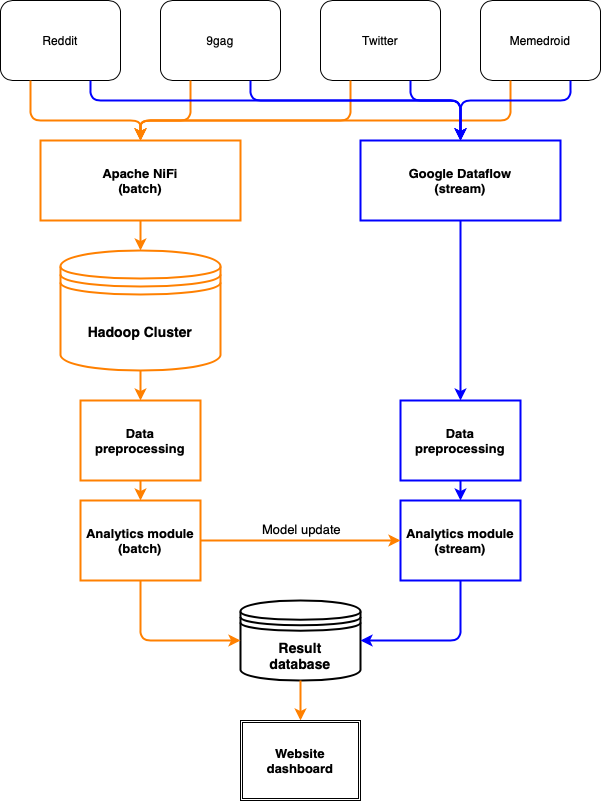
\includegraphics[scale = 0.50]{image.png}
\caption{'Project architecture'}
\end{center}
\subsection{Tools}
%używane technologię
\begin{itemize}
    \item Google Cloud Platform
    \item Apache NiFi
    \item Google Dataflow
    \item Hadoop Cluster
    \item Spark
    \item Python
    \item Django
    \item SQL (MariaDB)
    \item Google Cloud Vision

\end{itemize}

% modele analityczne itd

% Kluczowe założenia dotyczące modelu przetwarzania danych
% np. przetwarzanie wsadowe, przetwarzanie danych w trybie
% strumieniowym
\section{Data processing}
\subsection{Feature extraction}
The main task is to extract text from each meme. To achieve such result Google Vision will be used. Furthermore, data will be cleaned in order to avoid inappropriate content which might badly affect the later analysis. Moreover all duplicates will be removed. 

The whole process might take such form:
\begin{enumerate}
    \item extract each desired feature from JSON items,
    \item download pictures in according to given urls,
    \item remove pictures not considered as memes
    \item extract texts from pictures
    \item remove potential duplicates
    \item forward data to analytical segment
    
\end{enumerate}

\subsection{Data Analysis}
%rozpoznawanie tematyki na bazie treści mema, przy użyciu algorytmu OCR
The main task to be covered is to label each meme based on its content and format. To achieve such results OCRed content will be clustered and the most commonly used tags will be used as categories names. On the other hand Google Vision will perform clusterization of images to find the most popular formats for memes.



% Listę wykonawców i proponowane założenia dotyczące zasad
% podziału prac pomiędzy wykonawców
\section{Tasks}
The task to be performed within this project are:

\def\arraystretch{1.5}%
\begin{table}[]
    \centering
    \begin{tabular}{lcccc}
         Task & Michał & Jakub & Maciej & Krzysztof \\
         \hline
         Project Management & & & & \Checkmark \\
         Human Resources & & &\Checkmark & \\
         Data collecting & 9GAG & Twitter & Memedroid, 9GAG & Reddit \\
         Cloud initialization & \Checkmark & \Checkmark & \Checkmark & \Checkmark \\
         Apache NiFi, HDFS & \Checkmark & & \Checkmark &\\
         Google Dataflow & & \Checkmark & & \Checkmark \\
         Data Preprocessing & & & \Checkmark & \\
         Unit tests & \Checkmark & \Checkmark& \Checkmark & \Checkmark \\
         Advanced Analytics & \Checkmark & \Checkmark & \Checkmark & \Checkmark  \\
         Final Webapp & \Checkmark & & & \\
         Data Visualization & & &  & \Checkmark \\
         
    \end{tabular}
    \caption{Tasks distribution}
    \label{tab:my_label}
\end{table}

\end{document}
